\chapter{Xunzi}


\section{Xunzi, Maître Xun, 1ère moitié du IIIe siècle av. J.-C.}
 \begin{marginfigure}
     \centering
          \caption{Portrait de Xunzi}
     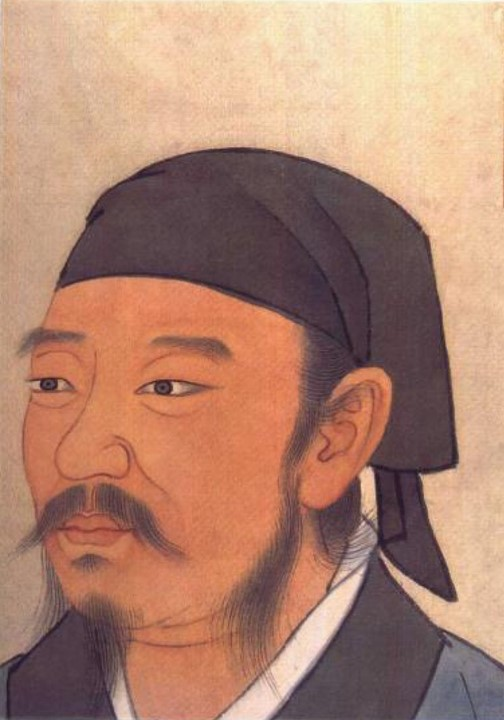
\includegraphics[width=\textwidth]{ConfucianismeTaoismeBouddhismeChinois/Images/Xunzi.jpg}

     \label{fig:enter-label}
 \end{marginfigure}
\begin{singlequote}
    Il a souvent été dit que Mencius et Xunzi représentent deux faces différentes mais complémentaires de l’héritage confucéen. Alors que le premier en présenterait la face idéaliste en confirmant le pari sur l’homme par sa conviction que la nature humaine est bonne, le second en ferait ressortir l\textbf{a face réaliste dans toute sa vigueur et sa rigueur.}
-- Anne Cheng, Histoire de la pensée chinoise, Paris: Seuil, 1997,
p. 212.

\end{singlequote}


\paragraph{Pays de Qi} le pays de Qi crée une académie  \textit{Jixia}pour les conseillers itinérants. Reconnaissance des \textit{shis}. Xunzi y enseigna et eut d'illustres d'élèves


\mn{texte : Ivan P. KAMENAROVIC, Écrits de Maître Xun, Paris : Les Belles Lettres, 2016.}


\paragraph{Style très différent} Chez confucius et Mencius, des dialogues et des conversations. L'oeuvre de Xunzi est de 32 chapitres, chacun avec un thème : "du ciel",... Les dialogues sont fictifs. Discours élaboré.

\section{Le ciel chez Xunzi}

\begin{Prop}
    Chez Mencius, un lien très fort entre l'homme et le ciel. \textit{connaitre sa nature, connaitre le ciel} : une proximité. 
    Pour Xunzi, la nature est des ressources mais pas de lien avec l'homme, pas de signe. L'homme doit faire sa propre loi car pas de volonté.
\end{Prop}


\begin{Def}[Ying - Yang]
    Deux formes d'énergie. Ying : lune, perle, nuit. Yang : soleil.
\end{Def}
Dans le livre des mutations, livre confucéen, livre de divination pour comprendre s'il faut être actif ou passif. Mais ce livre des mutations, est aussi un livre de \textit{perspicacité}, bonne analyse de la situation : ne pas aller à l'encontre des tendances. 
\begin{singlequote}
    1.	L’action du ciel est immuable, ce n’est ni l’attitude d’un Yao qui la fait subsister ni celle d’un Jie qui la fera cesser. Si on lui répond par l’ordre, le ciel nous est favorable et il nous est défavorable si on lui répond par le désordre. Si l’on renforce les activités de base et qu’on en use avec modération, le ciel ne saurait appauvrir. Si l’on a de quoi bien se nourrir et qu’on s’active selon la saison, le ciel ne saurait envoyer de maladies. Si l’on suit la voie sans dériver, le ciel ne saurait mander des catastrophes. Car, alors, les inondations et les sécheresses ne pourront pas susciter de famine, les grands froids et les canicules ne causeront aucun dommage, les mauvais présages et les phénomènes étranges ne pourront rien entraîner de funeste. Mais si l’on néglige l’agriculture et qu’on gaspille, le ciel ne pourra apporter aucune richesse, si la nourriture vient à manquer et qu’on se mette à la gaspiller, ce n’est pas le ciel qui y pourvoira, si l’on tourne le dos à la voie et qu’on se conduise en dépit du bon sens, le ciel ne saurait se montrer favorable. Dans ce cas, il n’y aura pas besoin d’inondations ou de sécheresses pour qu’il y ait des famines, il ne faudra ni gels ni canicules pour que surviennent les maladies et l’on connaîtra un sort néfaste sans que se soit produit aucun phénomène rare ou étrange. Les saisons, dans ce cas, se succèdent aussi bien que lors des périodes de bon gouvernement mais ce sont les catastrophes et les calamités qui surviennent différemment. On ne saurait en faire reproche au ciel mais bien à la voie qu’on aura suivie. Faire clairement la part de ce qui relève du ciel et de ce qui relève des humains, voilà qui est d’un homme vraiment complet.
-- Chapitre 17 « Du ciel », p. 227.
\end{singlequote}


Ce sont les actions qui comptent.


\begin{singlequote}
    2.	Le ciel a ses saisons, la terre a ses richesses, l’homme a sa gouverne, c’est à partir de là qu’il est possible pour eux de former ensemble une triade. Abandonner ce grâce à quoi l’on fait partie d’une triade tout en désirant en faire partie, cela est insensé. Le cours des astres et des étoiles, l’alternance du soleil et de la lune, le cycle des quatre saisons, l’alchimie du yin et du yang, le fait que les vents et les pluies se répandent en tous lieux, que chacun des dix mille êtres reçoive ce qui lui permet de venir harmonieusement au monde, d’y croître et d’y prospérer, nous n’en voyons pas les causes mais seulement les effets, alors nous qualifions cela de « divin ». Tout le monde saisit le processus d’accomplissement des phénomènes mais personne ne comprend ce qui ne revêt aucune forme, alors on l’appelle « l’œuvre céleste ». Seul le sage fait en sorte de ne pas chercher à connaître le ciel.
-- Chapitre 17 « Du ciel », p. 228.
\end{singlequote}

Pour nous, il y a le ciel, la terre et l'homme et chacun a son champ. L'homme doit s'interesser sur son domaine.
Il ne faut pas transgresser son propre domaine.

\section{La nature humaine est mauvaise}
\begin{singlequote}
    3.	La nature humaine est mauvaise et ce qu’il y a de bon dans l’homme est une élaboration. Il est naturel à l’homme d’aimer ce qui va dans son propre intérêt mais s’il suit ce penchant,
les querelles et les spoliations prospèrent au détriment de toute courtoisie et de toute civilité. L’homme est de naissance porté à la haine et à la jalousie mais s’il suit ce penchant, les torts et les dommages prospèrent au détriment de toute loyauté et de toute confiance. C’est de naissance encore que l’œil et oreille éprouvent le désir des couleurs et des sons mais si l’homme suit ces penchants, la licence et le désordre fleurissent au détriment des rites, de la morale, de la culture et du respect de l’ordre des choses.
 
Ainsi donc, pour peu que l’homme cède à sa nature et obéisse à la pression de ses inclinations, des querelles et des spoliations s’ensuivent nécessairement, on fait fi des différenciations sociales, on perturbe l’ordre des choses et l’on en retourne à l’état sauvage. C’est pourquoi il est nécessaire que les hommes soient civilisés grâce aux règles enseignées par les maîtres et qu’ils soient guidés par les rites et le sens moral pour qu’apparaissent la courtoisie et la civilité ainsi que la culture et le respect du cours naturel des choses, moyennant quoi l’on en arrive à l’ordre. Ces quelques observations montrent clairement que la nature de l’homme est mauvaise et que ce qu’il y a de bon en lui est le fruit d’une élaboration.
-- Chapitre 23 « La nature humaine est mauvaise », p. 321.

\end{singlequote}

Dans la nature humaine, Xunzi insiste bcp sur l'\textbf{élaboration} qui veut dire étymologiquement \textit{faux}. 

La moralité est quelque chose d'artificiel.

\begin{singlequote}
    4.	Mengzi a dit : « Si l’homme est capable d’apprendre, c’est donc que sa nature est bonne. » Je lui répondrai qu’il n’en est point ainsi, que c’est là bien mal connaître la nature humaine et ne pas savoir discerner ce qui, en l’homme, est naturel et ce qui est élaboré.
Ce qui est naturel est ce qui nous est spontanément donné par la céleste nature et cela ne peut pas s’apprendre ni se fabriquer. Quant aux rites et au sens moral, ils proviennent des sages, ils constituent ce dont l’homme est capable après l’avoir appris et qui ne porte ses fruits qu’au prix d’un travail accompli. Ce qui ne s’apprend ni ne se travaille mais qui est donné à l’homme est ce qu’on appelle sa nature. Ce dont l’homme n’est capable qu’après l’avoir appris et qui ne se trouve réalisé en l’homme qu’au prix d’un travail accompli est appelé élaboré. Telle est la différence entre le naturel et l’artificiel.
-- Chapitre 23 « La nature humaine est mauvaise », p. 323.


\end{singlequote}


On voit vraiment la différence radicale entre Xunzi et Mencius : \textit{préserver ce qu'on a déjà}. Alors chez Xunzi, il s'agit d'une transformation de l'homme de quelque chose qui n'existe pas naturellement. 


\begin{singlequote}
    5.	C’est pourquoi je dis que le naturel est racine, commencement, bois brut, alors que ce qui est élaboré est culture, expression de l’ordre des choses, élévation, enrichissement. Si le naturel n’est pas là, il n’y a rien à élaborer mais sans être élaboré, le naturel ne saurait briller par lui-même. C’est l’assemblage des deux qui fait le renom du sage et c’est grâce à lui que peut être menée à bien l’unification du monde. J’affirme donc que l’union du ciel et de la terre donne naissance aux dix mille êtres, que l’alternance du yin et du yang est le moteur de toutes les évolutions et transformations et que la combinaison du naturel et de l’élaboré permet au monde de se trouver ordonné.
-- Chapitre 19 « Des rites », p. 270.
\end{singlequote}

\subsection{Yin et Yang}

Dans le Livre des mutations (ou Classique des changements), le yin, représenté par un trait brisé et le yang, par un trait continu, forment les huit trigrammes.


Deux trigrammes superposés engendrent un hexagramme. Les 64 hexagrammes constituent les éléments centraux du Livre des mutations. 

\section{L’étude}

La première compétence, c'est l'étude. pour Xinzu, il s'agit de transformation. Paradoxal, car il est certes mauvais, mais il peut se transformer. L'homme devient l'homme avec la \textbf{culture}.

\begin{singlequote}
    6.	Par quoi commence l’étude et par où finit-elle ? Je dirais qu’elle débute par la récitation des Classiques et qu’elle se termine par la lecture des Rites. Son but est de commencer par former des hommes capables et, à son terme, de former des sages. Ce n’est qu’au prix d’efforts réitérés qu’on parvient à quelque chose et l’étude ne saurait prendre fin qu’avec la mort. Si l’art d’étudier a une fin, elle est que l’étude ne se relâche pas un seul instant. \textbf{Qui s’y adonne est vraiment un homme, qui l’abandonne n’est qu’une bête.}
-- Chapitre 1, « Exhortation à l’étude », p. 6.
\end{singlequote}

On fait des hommes \textit{capables} avant d'en faire des \textit{sages}.


\begin{singlequote}
    7.	Je me suis essayé des journées entières à penser par moi-même, cela ne vaut pas un seul instant consacré à l’étude. J’ai essayé de me dresser sur la pointe des pieds, cela ne vaut pas l’ascension d’une montagne d’où l’on jouit d’une large vue. S’élever pour faire un signe n’allonge pas le bras, mais cela permet d’être vu de plus loin. Crier dans le sens du vent ne renforce pas la voix mais permet d’être entendu plus distinctement. Emprunter une voiture à cheval ne fait pas mieux marcher mais permet de parcourir des li1 par milliers. Monter en barque et ramer ne fait pas
\mn{1 La longueur du li était à l’époque d’environ 400 mètres. [Note du traducteur]}
 mieux nager mais aide à traverser fleuves et rivières. Ainsi, l’homme accompli n’a-t-il rien de particulier à la naissance, si ce n’est qu’il possède l’art du bon usage des choses.
-- Chapitre 1 « Exhortation à l’étude », p. 2.
\end{singlequote}



\begin{singlequote}
    8.	C’est par l’écoute que l’étude pénètre en l’homme accompli, elle se manifeste en son cœur et s’exprime dans tout son corps. Il en témoigne aussi bien par son activité que par son repos. La moindre parole qu’il murmure, le moindre geste qu’il esquisse peuvent être des exemples pour autrui. Chez l’homme de peu, à peine l’étude a-t-elle pénétré par l’oreille, que déjà elle ressort par la bouche et pourtant de l’une à l’autre il n’y a que quatre pouces. Comment cela suffirait-il pour rendre admirable un homme de sept pieds de haut ? Les anciens étudiaient pour eux-mêmes, nos contemporains le font pour les autres.
-- Chapitre 1 « Exhortation à l’étude », p. 6.
\end{singlequote}



\begin{singlequote}
    9.	La terre s’amassant en collines fait lever le vent et la pluie. Les eaux s’accumulant en des fosses profondes font naître crocodiles et dragons. La pratique constante du bien fait naître la vertu. C’est ainsi qu’on obtient les lumières de l’esprit et qu’on se fait le cœur d’un sage. Si l’on n’ajoute pas une enjambée à l’autre, on ne parcourra jamais mille li et sans une succession de petits ruisseaux il ne se formerait ni fleuves ni mers. Un pur-sang ne franchira pas dix pas d’un seul bond, tandis qu’un solide cheval pourra franchir de longues distances sans se décourager. Si on laisse en plan son entaille, on ne coupera pas même du bois mort mais si l’on persévère, on taillera le métal et la pierre. Le ver de terre n’a pour lui ni le mordant des griffes et des dents ni la puissance des muscles et des os, il rampe dans la poussière pour se nourrir et descend s’abreuver jusqu’aux Sources jaunes\sn{Là où séjournent les morts dans la tradition antique. [Note du traducteur]}, l’esprit tendu vers un seul but. Pourvu de six pattes et de deux pinces, le crabe, à moins de s’introduire dans l’antre d’une anguille, n’a pas même un trou où habiter ni se cacher car son esprit est trop agité. Ainsi, l’on ne saurait, sans suite dans les idées, avoir l’esprit clair et, faute d’affronter des affaires complexes, on ne saurait jouir d’un succès mérité.
-- Chapitre 1 « Exhortation à l’étude », p. 4.
\end{singlequote}
Les étudiants apprennent le 9 par coeur. 
Le dragon est un être merveilleux dans la tradition chinoise.



\section{Les rites
}

Avoir sa propre place dans la société : rôle des rites


\begin{singlequote}
    10.	D’où proviennent les rites ? La réponse est que les hommes naissent avec des désirs. Si ces désirs sont insatisfaits, il ne peut pas ne pas y avoir d’exigences. Si ces exigences sont sans retenue, sans mesure, sans partage et sans limite, il ne peut pas ne pas y avoir de conflits. Or, les conflits engendrent le désordre et celui-ci, la misère. Les anciens rois, par aversion pour le désordre, instituèrent les rites et le sens moral afin de procéder à des répartitions, de nourrir les désirs des humains et de répondre à leurs exigences. Ils ont fait en sorte que les désirs n’aillent point excéder les objets désirés et que ceux-ci ne viennent point manquer aux désirs. Faire régner entre les deux un durable équilibre, voilà ce qui a présidé à la naissance des rites.
-- Chapitre 19 « Des rites », p. 257.
\end{singlequote}

Décret très connu pendant les Han. 



11.	Or l’homme a l’énergie, il a la vie, il a la conscience à quoi s’ajoute le sens du devoir, c’est pourquoi il est le plus noble de tout ce qui est sous le ciel. Sa force est moindre que celle du buffle et sa vitesse moindre que celle du cheval et pourtant il se sert du buffle et du cheval. Comment cela se fait-il ? C’est que l’homme est capable de se constituer en société, ce dont les autres ne sont point capables. Et comment se constitue-t-il en société ? Par la répartition [sociale des tâches]. Comment cette répartition peut-elle fonctionner ? Grâce au sens du devoir. Car c’est ce sens des devoirs rituels combiné à la répartition des tâches qui permet de vivre dans la concorde et la concorde à son tour permet l’unité. Cette unité fait se rassembler les forces qui donneront la puissance nécessaire pour dominer les choses. Alors l’homme peut avoir des palais et des maisons pour habitations, il respecte l’ordre des saisons et régente les dix mille êtres, il jouit des avantages de tout ce qui est sous le ciel et cela sans autre cause que la répartition des tâches et l’équité des devoirs rituels. C’est pourquoi l’homme, dès sa naissance, ne peut faire autrement que de s’intégrer à une société. Si cette société ne procède pas à une répartition des tâches, elle sera en proie à des conflits qui la mèneront au désordre, lequel sera cause d’éclatement, donc de faiblesse et, partant, de l’impossibilité d’assurer sa prédominance sur les choses.
-- Chapitre 9 « De l’œuvre royale ».
